\section{Analyse des Schaltplans vom Empfänger} %Erik

\section{Vorverstärkung des Signals} %Lukas

\section{Frequenz-Downkonversion} %Farhad
Im Folgenden wird die Frequenz-Downkonversion des analogen Signals, der bereits vor dem Eingang in den Downconverter verstärkt wurde, erklärt.
\subsection{Ablauf der Frequenz-Downkonversion in der Schaltung}
In der Abbildung \ref{fig:downconverter} ist die Schaltung des Downconverters zu sehen.
\begin{figure}[H]
    \centering
    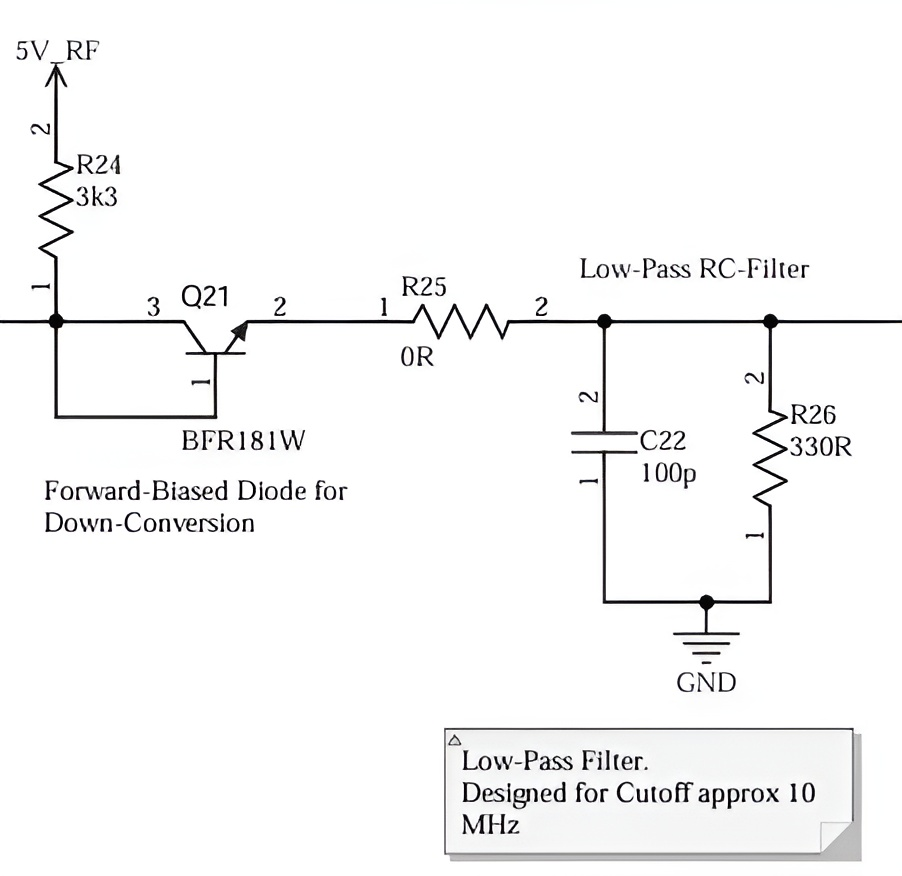
\includegraphics[width=0.8\textwidth]{Pictures/Downconverter.png}
    \caption{Schaltung des Downconverters}
    \label{fig:downconverter}
\end{figure}
Dieser Downconverter stellt einen einfachen Abwärtsmischer dar, der dazu dient, einen hochfrequenten \ac{RF}-Einganssignal in ein niederfrequentes Ausgangssignal umzuwandeln. 

Zuerst gelangt das hochfrequente Signal in den Transistor Q21 (BFR181W), der in dem Fall nicht als Verstärker, sondern als Diode betrieben wird, da die Basis und der Kollektor dessen verbunden sind. Somit wird effektiv nur die Basis-Emitter-Strecke des Transistors benutzt. Dieser Transistor ist ein \textbf{nichtlineares} Baulement.
Ein nichtlineares Bauelement wird zum Mischvorgang in diesem Zusammenhang benötigt, da es die Amplitudenmodulation des Signals ermöglicht. 

An den Eingang des Mischers, also des Transistors Q21, werden zwei Signale angelegt: das eigentliche \ac{RF}-Signal, welches in diesem Fall bei 1,25 GHz liegt, und ein \ac{LO}-Signal.

Wenn die beiden Signale die vorgespannte Diode passieren, erzeugen diese aufgrund der nichtlinearen Eigenschaften des Transistors eine Mischung der beiden Signale. Die neuen Frequenzen sind hierbei die Summe $f_{RF} + f_{LO}$ und die Differenz $f_{RF} - f_{LO}$ der Eingangsfrequenzen. 
Da hier eine \textbf{Abwärtsmischung} erwünscht ist, wird die Frequenz $f_{RF} - f_{LO}$ weiterverarbeitet. 
Nach der erfolgreichen Abwärtsmischung des Signals kommt es zu einer Signalfilterung. Dazu wird direkt nach dem Transistor Q21 ein RC-Tiefpassfilter geschaltet, der die Frequenz $f_{RF} + f_{LO}$ herausfiltert und nur das niederfrequente Differenzsignal $f_{RF} - f_{LO}$ passieren lässt. Der Filter besteht aus den Bauelementen R26 ($330~\Omega$) und C22 ($100~\mathrm{pF}$). Der Kondensator ist dabei so dimensioniert, dass der Filter insgesamt eine Grenzfrequenz von $f_{c} = 10~\mathrm{MHz}$ aufweist. Die widerspricht zwar dem rechnerischen Wert, der sich aufgrund der Werte von R26 und C22 ergibt, also $f_{c, rechnerisch} = \frac{1}{2\pi R C} = 4,8~\mathrm{MHz}$, lässt sich jedoch durch Vereinfachungen im Schaltplan oder den Fakt, dass hier ein idealer Tiefpassfilter angenommen wird, erklären. Außerdem ist es bei hohen Frequenzen zu beachten, dass die Leiterbahnen in der Schaltung parasitäre Effekte aufweisen (in Form von Induktivitäten und Kapazitäten), die ebenfalls die Grenzfrequenz beeinflussen können. Diese wurden in der oben ausgeführten Berechnung nicht berücksichtigt.

\subsection{Funktion des Widerstandes R\textsubscript{24}}
Dabei ist zu beachten, dass der Transistor durch den Widerstand R24 auf eine Spannung von 5V vorgespannt wird. Die Aufgabe dieses Widerstandes ist es, den richtigen Arbeitspunkt für den Transistor Q21 zu setzen, damit dieser im Mischbetrieb arbeiten kann. Er begrenzt den Gleichstrom, der von der 5V-Versorgungsspannung zum Transistor fließt, und stellt sicher, dass der Transistor im aktiven Bereich arbeitet. Dadurch wird eine optimale Signalverarbeitung ermöglicht, da der Transistor in der Lage ist, die Modulation des Signals korrekt zu erfassen und weiterzuleiten. Ohne diesen Widerstand könnte der Transistor übersteuert werden, was zu Verzerrungen im Signal oder zur Zerstörung des Transistors führen würde.


\section{Operationsverstärkerschaltung} %Lukas 5a und c

\section{Komparatorschaltung} %Erik 6 a und b
\clearpage